\documentclass{article}
\title{CSC231 Project1}
\author{Alex Zhang}
\date{October 2023}
\textwidth=16.00cm 
\textheight=22.00cm 
\topmargin=0.00cm
\oddsidemargin=0.00cm 
\evensidemargin=0.00cm 
\headheight=0cm 
\headsep=0.5cm
\textheight=610pt
\usepackage{graphicx}
\usepackage{multicol}

\usepackage{relsize}




\graphicspath{ {./images/} }

\usepackage{latexsym,array,delarray,amsthm,amssymb,epsfig}
\usepackage{amsmath}
\usepackage{listings}
\lstset{
  basicstyle=\ttfamily,
  mathescape
}


\newcommand{\bmat}[1]{\begin{bmatrix} #1 \end{bmatrix}}
\newcommand{\mat}[1]{\mathbf{#1}}

\let\ds\displaystyle

\begin{document}
\maketitle
The following figure is the graphical representation of my finite state machine.
\begin{figure}[!ht]
    \begin{center}
        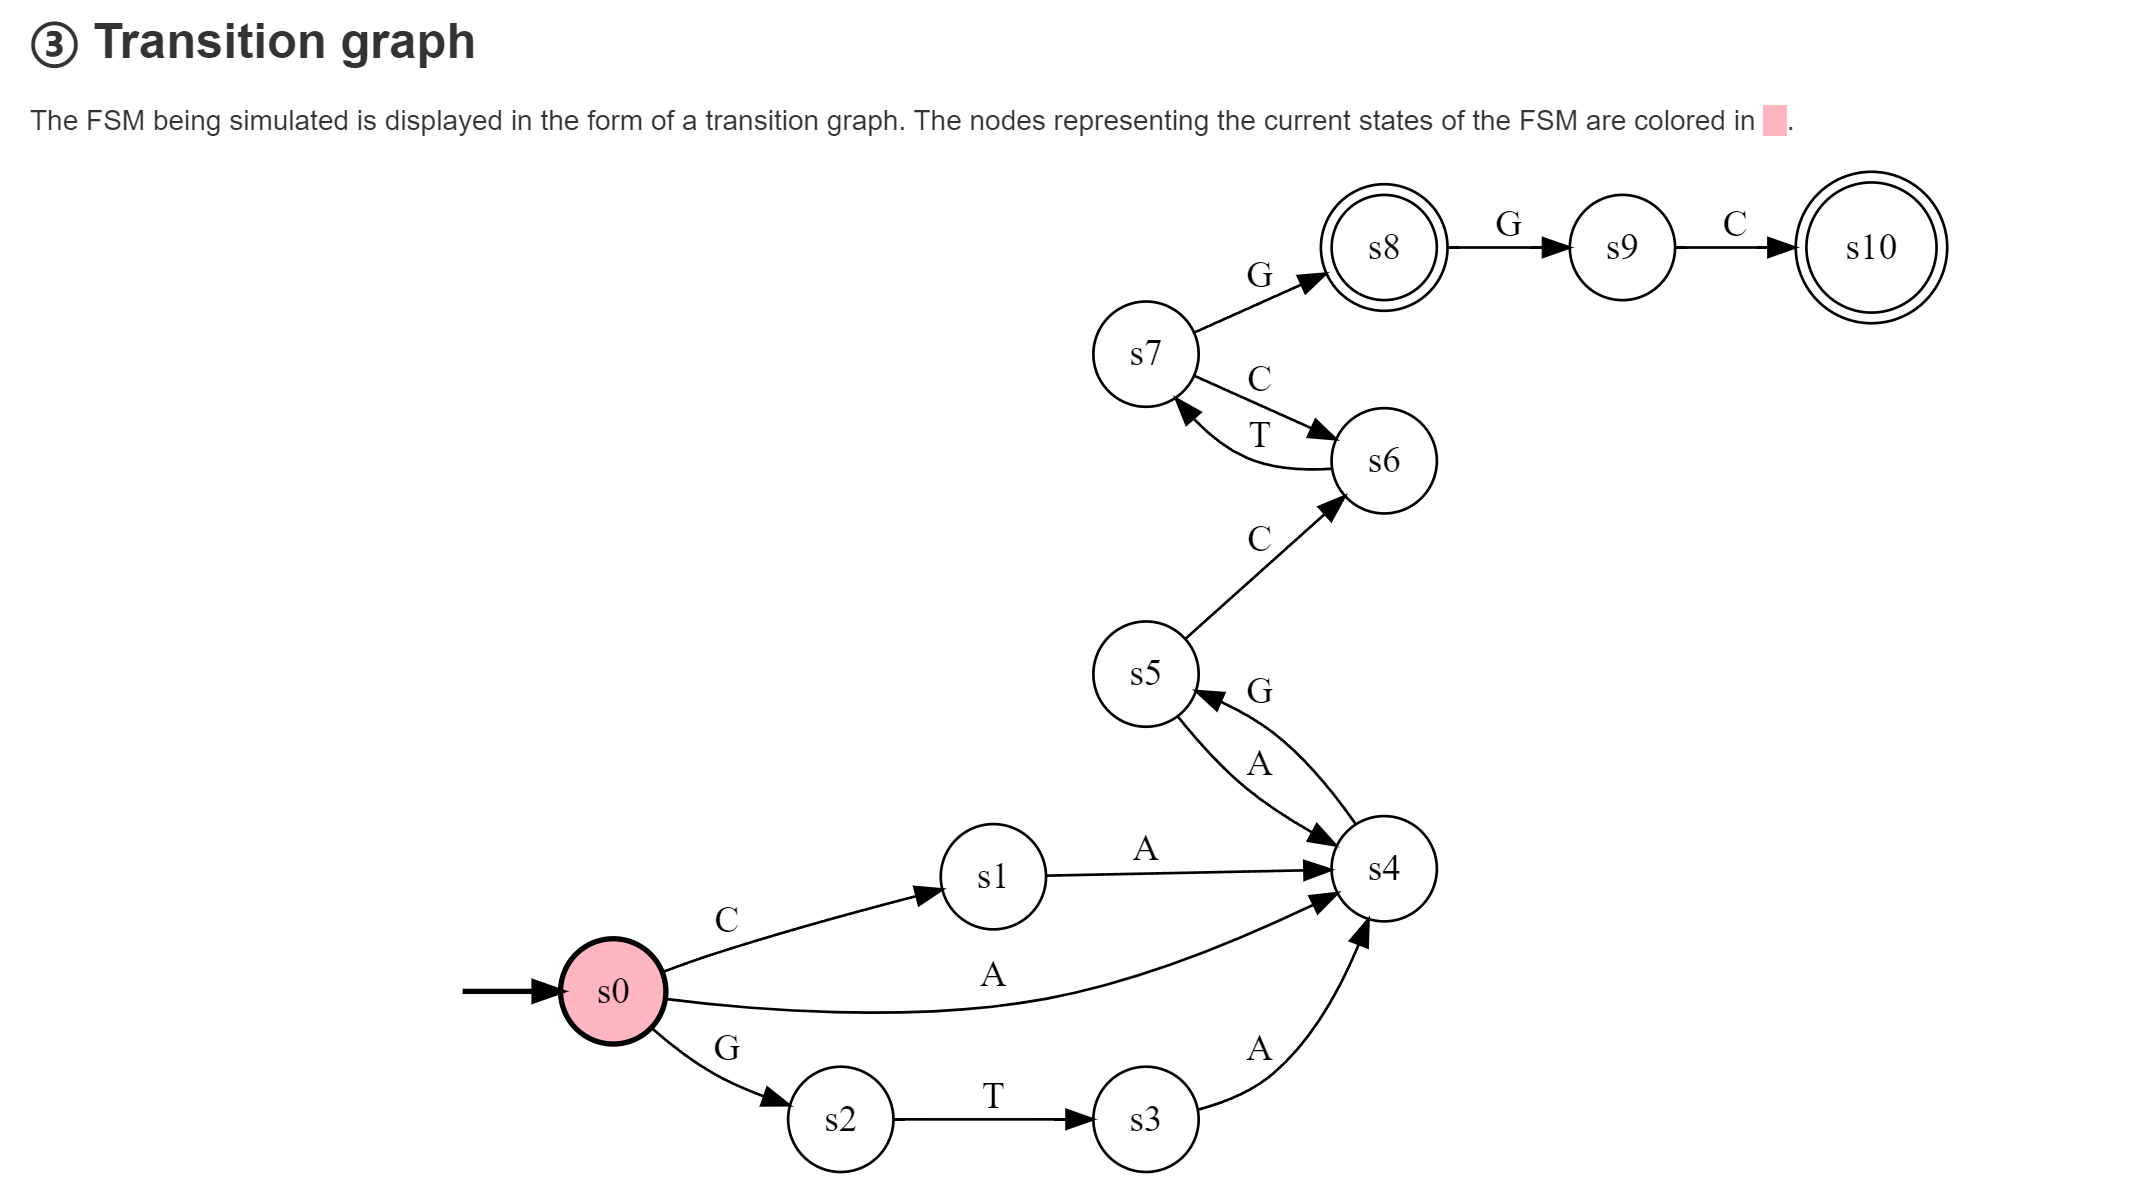
\includegraphics[scale = 0.5]{DFSM.png}
    \end{center}
\end{figure}
\section*{Explanation}
Based on the figure, s0 is the starting state. I did not include an explicit trash state but every letter in each state without rules goes into trash state.
\begin{enumerate}
    \item s1 state checks the optional C at the beginning of the words
    \item s2 and s3 check the optional GT at the beginning of the words.
    \item s4 and s5 is the loop that check containing one or more instances of AG.
    \item s6 and s7 use the loop to check whether contains one or more instances of CT.
    \item s8 checks whether it contains only one G.
    \item s9 and s10 check the optional GC at the end of the words.
\end{enumerate}
\section*{Three Additional Words}
Three additional words that are in part of the language will be:
\begin{enumerate}
    \item GTAGAGAGCTCTCTG
    \item AGAGCTCTGGC
    \item AGCTGGC
\end{enumerate}

Three additional words that are NOT part of the language will be:
\begin{enumerate}
    \item T
    \item GTAGCTT
    \item GTAGCTCTGGT
\end{enumerate}










\end{document}